\documentclass[14pt,a4paper,oneside]{article}

\usepackage[utf8]{inputenc}   


\usepackage{amsmath,amsthm,amssymb,appendix,bm,mathrsfs,ctex,geometry,tcolorbox,fancyhdr,tikz,esint,appendix}


%% GB/T 7714 宏包 ---- 引文格式
\usepackage[sort&compress]{gbt7714}
\bibliographystyle{gbt7714-numerical}



\numberwithin{equation}{subsection}             %%%%%% 公式编号




\geometry{left=1.7cm, right=1.7cm, top=2.54cm, bottom=2.54cm}    %%%%% 页面尺寸
\linespread{1.5}                             %%%%% 行距1.5倍
\pagestyle{fancy}



%%    设置页眉页脚
\fancyhf{}
\renewcommand{\headrulewidth}{0.15mm}
\fancyhead[C]{文献阅读报告}                   %%%%%% 页眉
\fancyfoot[C]{\thepage}                      %%%%%% 页脚 页码
\setlength{\headheight}{15pt}


%%   设置各种链接颜色为黑色
\usepackage[colorlinks,
            linkcolor=black,
            anchorcolor=black,
            citecolor=black,
            urlcolor=black
            ]{hyperref}



%%   例子编号
\newcounter{example}
\counterwithin{example}{subsection}
\newcommand{\examplename}{Example}
\newcommand{\exampleTitle}[1]{%
\textbf{\refstepcounter{example}\examplename\theexample:#1}\par}


%%  插入图片配置
\usepackage{graphicx,subfigure}
\usepackage[]{caption2} %新增调用的宏包
\numberwithin{figure}{subsection}               %%%%%% 图片编号

\graphicspath{ {./Figure/} }            %%%%% 设置图片文件所在目录
\DeclareGraphicsExtensions{.pdf,.svg,.jpeg,.png,.jpg}     %%%%% 支持图片格式


%%    支持tikz作图
\usepackage{tikz}
\usetikzlibrary{backgrounds,arrows}


\usepackage{pgfplots}
\pgfplotsset{compat=1.15}
\usepackage{mathrsfs}


\title{\textbf{文献阅读报告 4\\Operation at 1 MHz of 1.7-cycle multiple plate compression at 35-W average output power}}                           %%%%% 标题
\author{骆禹天}                                           %%%%% 作者
\date{2024/**/**}                                        %%%%%% 日期

%%   定义一些数学格式
\newtheorem{theorem}{定理}[subsection]
\newtheorem{definition}[theorem]{定义}
\newtheorem{lemma}[theorem]{引理}
\newtheorem{corollary}[theorem]{推论}
\newtheorem{example}[theorem]{例}
\newtheorem{proposition}[theorem]{命题}
\renewcommand{\abstractname}{\Large\textbf{摘要}}




%------------------------- 开始文档  -------------------------%



\begin{document}

\pagenumbering{Roman}         %%%%% 目录前页码统计按罗马数字

\maketitle

\setcounter{page}{1}          %%%%% 标题开始统计页数

%------------------------- 目录  ------------------------------%

\tableofcontents              %%%%% 插入目录

\newpage                      
\setcounter{page}{1}          %%%%% 目录后重新统计页数


\pagenumbering{arabic}        %%%%% 目录后统计页码为阿拉伯数字



%%%%%%%%%%%%%%%%%%%% 开始第一节  %%%%%%%%%%%%%%%%%%%%%



\section{Introduction}

\subsection{超短脉冲应用}

超短脉冲的光谱展宽和压缩可实现高脉冲加宽和压缩因子并产生少周期电场. 应用: 

(1) 超快泵浦-探针光谱\cite{pashkinElectricMagneticTerahertz2013};

(2) 纳米复制;\cite{planklSubcycleContactfreeNanoscopy2021}

(3) 阿秒科学;\cite{corkumAttosecondScience2007}

(4) x射线或XUV源\cite{klasUltrashortpulseHighaveragepowerMegahertzrepetitionrate2021, teichmann5keVSoftXray2016}.

\subsection{多通腔}

多通腔中, 脉冲多次通过腔内非线性介质, 可大大增加光束的传播距离, 用于光谱展宽和脉冲压缩。Herriott腔相较光纤的优势:

(1) 更不容易错位, 

(2) 高峰值和平均功率下更不易损坏。固体与气体多通腔分别覆盖了9 MW\cite{weitenbergMultipasscellbasedNonlinearPulse2017a}至81 GW\cite{kaumannsSpectralBroadening1122021}的输入峰值功率范围。

(3) 便携紧凑的结构.

Herriott腔相较光纤目前的难题: 难以支持必要的带宽以及管理腔镜的色散. --- 本文的科学问题: 如何管理多通腔腔镜的色散?

相较光纤利用全内反射而原则上不受光谱带宽限制, 多通腔腔镜需要金属或电介质涂层。

(a) 金属涂层有宽带宽且无色散, 但其每次反射有约百分之几的显著吸收损失。

(b) 介质镜带宽接近一个倍频程, 只有0.1\%量级的损耗, 并且还显示出群延迟色散（GDD）振荡。

不过即使光纤可支持极端带宽, 有效压缩到几个周期以下也需要出色的色散控制。这反过来又需要色散镜补偿更高阶色散。例如, 这可在光场合成器中实现\cite{wirthSynthesizedLightTransients2011}。

原则上具有不同的光谱通道在多通腔中展宽诸如此类的概念是可行的, 但实现起来复杂繁琐。

作者总结对比了多通系统中的一些结果见下表.

\begin{table}[!ht]
    \renewcommand{\arraystretch}{3}
	\centering\fontsize{9pt}{3}\selectfont
    \caption{多通系统输出低于20 fs脉冲结果总结与对比}
    \begin{tabular}{lccccccc}
    \hline
    & 单位 & 本工作 & 引用工作1\cite{fritschAllsolidstateMultipassSpectral2018} & 引用工作2\cite{mullerMultipassCellHighpower2021} & 引用工作3\cite{goncharovFewcyclePulseCompression2023a} & 引用工作4 & 引用工作5\cite{ballaPostcompressionPicosecondPulses2020a}\\
    \hline
    $P_{\mathrm{pk\;input}}$ & MW & 48 & 14 & 4700 & 105 & 21 & 1567\\
    $P_{\mathrm{pk\;output}}$ & MW & 1025 & 60 & $60,000^b$ & - & - & -\\
    $\tau_{\mathrm{pk\;input}}$ & fs & 230 & 220 & 200 & 1000 & 265 & 1200\\
    $\tau_{\mathrm{pk\;output}}$ & fs & 7 & 16 & 7 & 11 & 18 & 13\\
    $P_{\mathrm{avg\;input}}$ & W & 12 & 100 & 500 & 112 & 100 & $200^c$\\
    $P_{\mathrm{avg\;output}}$ & W & 10 & 60 & 388 & 15 & 61 & $37^c$\\
    Transm. & \% & 84 & 60 & 78 & 47 & 61 & 37 \\
    $f_{\mathrm{rep}},$ & MHz & 1 & 28 & 0.5 & 1 & 16 & 0.1 \\
    \hline
    \end{tabular}
\end{table}

\subsection{总结与意义}

本文作者依赖850-1300 nm带宽的色散镜和氩气作为非线性介质。由于电介质反射镜, 实现多通腔内平均功率扩展, 并且输出高质量脉冲(80\%的能量保留在主峰中, 整体透过率达到84\%)。此外, 作者依靠气体介质和色散介电涂层的组合实现精确的色散管理可控制MPC在正常、零或反常色散下工作，从而达到最佳的展宽和白光生成。最终在简单稳健的几何结构中，使用 fs 种子脉冲达到几个周期的脉冲持续时间以及 33 的高时间压缩因子。

潜在应用:

(1) 通过惰性气体中高次谐波产生（HHG）高重复率极紫外源\cite{klasUltrashortpulseHighaveragepowerMegahertzrepetitionrate2021}, 用于角分辨光电发射光谱（ARPES）\cite{puppinTimeandAngleresolvedPhotoemission2019} 或XUV频率梳光谱;

(2) 近红外多光子显微镜\cite{mojzisovaWhenMultiphotonMicroscopy2011} (峰值功率相当低, 最佳重复率在几MHz范围), 如高光谱多光子显微镜\cite{baresHyperspectralMultiphotonMicroscopy2020}, 它允许使用单个超宽带激光源同时激发不同的发色团。



\section{Method}

\subsection{Set up}

第一级: 

· 驱动激光器: Pharos 激光器，输出 1 MHz, 能量 12 $\mathrm{\mu J}$ 的，平均功率 12 W, 230 fs 脉冲。

· 第一个多通腔: 高反射镜曲率半径 150 mm和 100 mm, 间隔 190 mm;  3 mm厚涂有增透膜的熔融石英，距离输入镜约 10 厘米。 30 通产生总 B 积分 12.9 rad (每通 0.43 rad)。空气中运行。

· 色散镜反射9次压缩脉冲至 40 fs，由，每次反射 -400 $\mathrm{fs^2}$  GDD。由 SPIDER (APE GmbH) 检测。

第一级的透射率 94\%，主要归因于增透膜熔融石英的损耗。

第二级: 

· 一对互补色散镜, 曲率半径 200 mm，间隔为 380 mm. 充氩气。外壳有一个镀增透膜的熔融石英输入窗口。通数: 26。

· 氩的GVD约0.015$\mathrm{fs^2/mm}$, 腔镜设计为在 1030 nm左右两次反射提供约−100 $\mathrm{fs^2}$. 由不同气压，可调节多通腔在正常、零或反常色散状态工作. 压强 ~8.5 bar 为过渡值.

\begin{figure}[h]
    \centering
    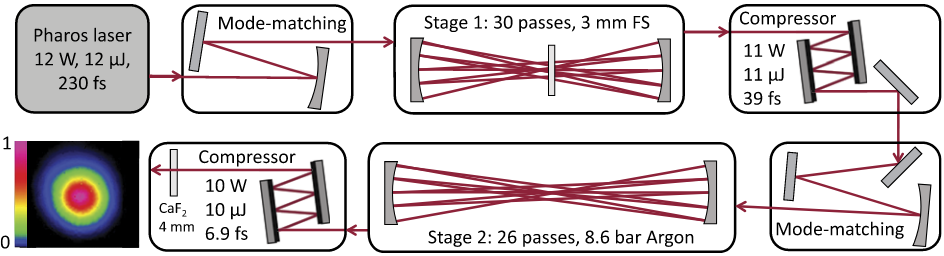
\includegraphics[width=0.6\textwidth]{p1.png}
    \caption{实验配置}\label{p2.1.1}
\end{figure}

\subsection{Simulation}

· 使用 PyNLO (https://github.com/pyNLO/PyNLO) 对非线性薛定谔方程进行数值求解.

· 网格包含 $2^{14}$ 个点, 时间窗口为 20 ps 。

· 该算法每次迭代都包含在一个方向上通过多通腔的 50 个步骤, 考虑了氩气的正色散以及焦散的形式。

· 然后，将腔镜的负色散作用于脉冲。算法还考虑了腔镜的透射曲线。

· 这个程序能紧密匹配实验条件。


%--------------------  第三节 结果  --------------------%


\section{Result}

\subsection{第一级} 

SPIDER测得输出脉冲被压缩到40 fs, 如图\ref{p3.0.1}, 与傅里叶极限比较: 主峰包含96\%的脉冲能量. 

\begin{figure}[h]
    \centering
    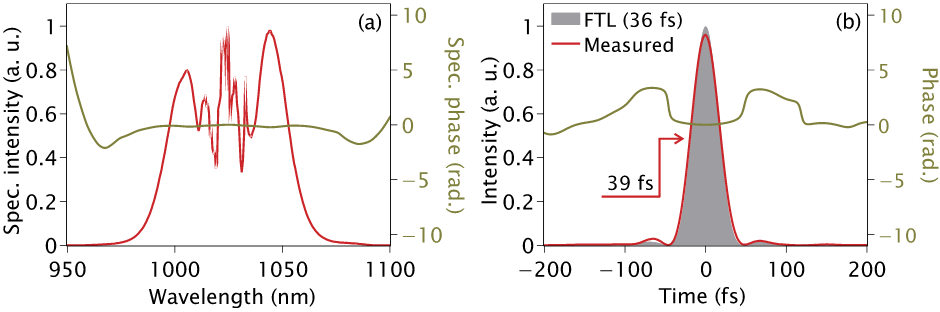
\includegraphics[width=0.6\textwidth]{p2.png}
    \caption{SPIDER 测量第一级输出脉冲: (a)  频域强度和相位; (b) 时域强度和相位, 与傅里叶极限比较}\label{p3.0.1}
\end{figure}

通过孔径200 $\mathrm{\mu m}$多模光纤耦合到光谱仪中测量光束不同位置光谱来表征空间光谱均匀性, 如图\ref{p3.1.2}. 重叠参数\cite{weitenbergMultipasscellbasedNonlinearPulse2017a}用于量化测量 [图\ref{p3.1.2}（a）]. 在光斑中心有>99\%的良好重叠，边缘处下降到90\%（定义为$1/e^2$），而加权平均值分别在$V_x=99\%$和$V_y=99\%$附近。

输出光束具有出色的质量，根据 ISO 11146 测量为 $M_2 = 1.2 \times 1.2$ [图\ref{p3.1.2}(b)]。与驱动激光 $M_2 \leq 1.2$ 相当。

\begin{figure}[h]
    \centering
    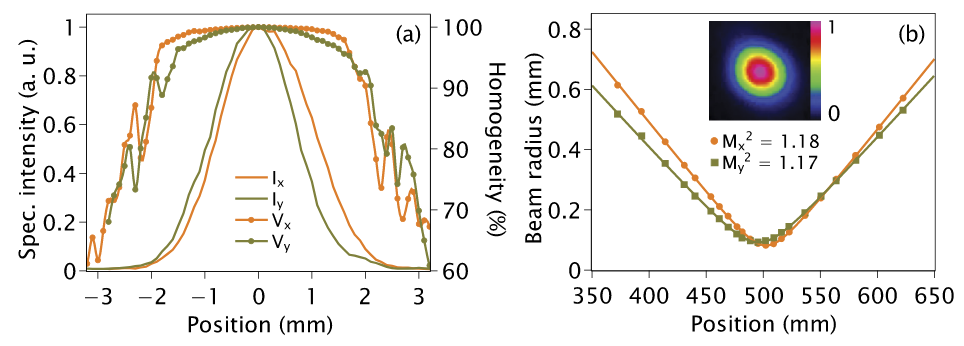
\includegraphics[width=0.6\textwidth]{p3.png}
    \caption{第一阶段输出空间光谱均匀性。 (a) 切向和矢状面的 V 和相对强度 I。 (b) 根据 ISO 11146 的光束质量测量 M2。点和线分别代表实验数据和拟合, 焦平面光束如插图所示。}\label{p3.0.2}
\end{figure}

\subsection{第二级} 

\subsubsection{正色散状态} 

第二级正色散状态, 对应压强 8.6 bar。这使宽带反射镜的整个带宽（850-1300 nm）能被充分利用，几乎不牺牲整体吞吐量. 

根据SPIDER测量, 主峰包含 80\% 的能量或~1.0 GW 峰值功率, 对应 33 倍的时间压缩和 21 倍的峰值功率增加。正色散状态下的第二级吞吐量为 89\%，基本由腔镜镀层决定，两级总透射率保持在 84\%。

根据测量的光谱计算出 6.5 fs 的傅里叶变换极限。输出脉冲通过色散镜 的四次反射 ($4 \times -45 \;\mathrm{fs^2}$) 和 4 mm厚的 $\mathrm{CaF_2}$ 窗口压缩至 7 fs。

没有观察到输出光束明显恶化（见图 \ref{p2.1.1}）。CCD 测得的光束质量参数为 $M_2 = 1.2 \times 1.2$表明通过级联多通腔光束没有衰减。

\begin{figure}[h]
    \centering
    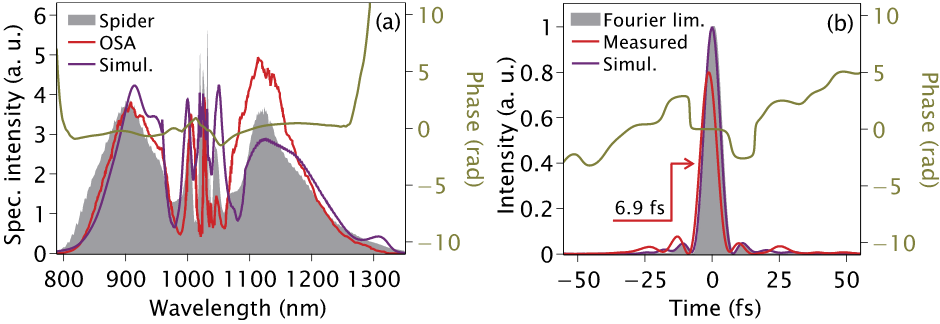
\includegraphics[width=0.6\textwidth]{p4.png}
    \caption{第二阶段正色散下的时域特征: (a) SPIDER 测量光谱相位（橄榄色）和强度（灰色）。另外用光谱分析仪（OSA）测量光谱。紫色为数值计算输出光谱。 (b) 与傅立叶极限 (6.5 fs) 比较: 主峰包含80\%能量.}\label{p3.2.1}
\end{figure}

同样方法表征输出光束的空间光谱均匀性[图\ref{3.2.2}]。光束中心（定义为 $1/e^2$）完美光谱重叠 >99\% ，边缘则降至 90\%。重叠因子的加权平均值分别为$V_x = 99\%$和$V_y = 99\%$。空间上光谱分布均匀良好。

13 h的长期功率稳定性测量表明功率长期稳定. [图\ref{p3.2.2}(b)]

\begin{figure}[h]
    \centering
    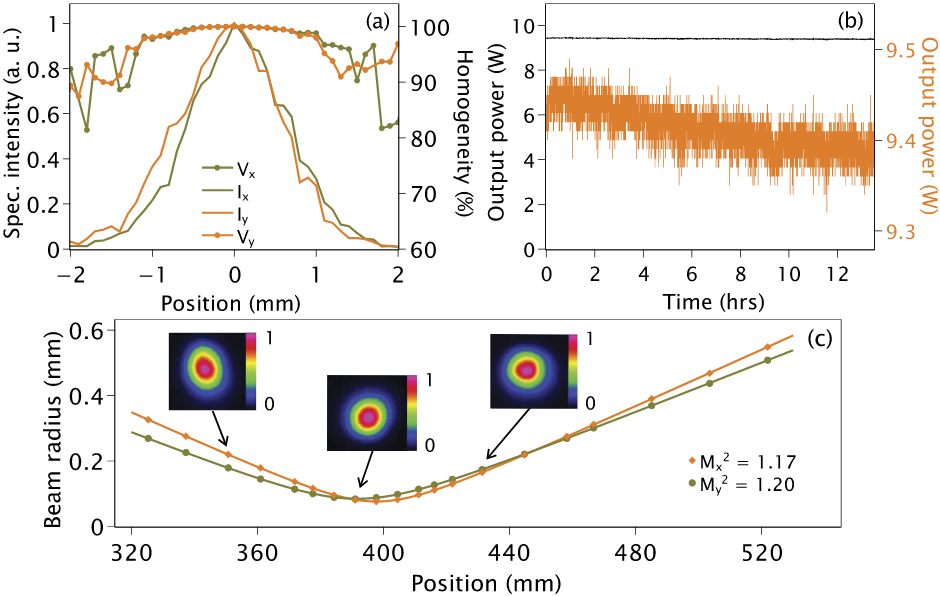
\includegraphics[width=0.6\textwidth]{p5.png}
    \caption{第 2 级输出表征。 (a) 切向平面和矢状平面的空间光谱均匀性 V 和相对强度 I。 (b) 输出功率长期测量。 (c) 光束质量 $M_2$ 测量。 878 nm 的中心波长根据 CCD 传感器的灵敏度进行平均加权。插图表示焦散内不同位置的光束轮廓。}\label{p3.2.2}
\end{figure}

\subsubsection{反常色散状态}

将气压微调至 8 bar, 氩气正色散被腔镜负色散稍微过度补偿达到净反常色散状态。

反常色散导致腔内脉冲部分自压缩，并能够在当前配置下最大化地展开光谱。输出光谱达到整个倍频程覆盖了 700-1450 nm 范围。该实验表明，使用多通腔可实现倍频程带宽并最终输出白光。

然而，由于宽带腔镜超出工作范围线性损耗较高，总吞吐量降低到 <80\%。

作者将测量光谱翼中的调制归因于 MPC 反射镜在其工作区域之外的色散分布.

\subsection{Simulation}

通过Pylno进行数值模拟, 实验结果与数值模拟吻合良好。考虑到理论上跨越一个倍频程的宽带反射镜的平坦色散（GDD为−50 $\mathrm{fs^2}$）和透射曲线（∼0.1\%），我们将模拟扩展到实验条件之外，以展示光谱展宽和透射率的前景。多通腔中脉冲压缩, 如图\ref{p3.3.1}所示，可高效（>90\% 吞吐量）实现跨整个倍频程产生，为实现 FTL < 5 fs 的可压缩亚 2 周期系统铺平道路。

\begin{figure}[h]
    \centering
    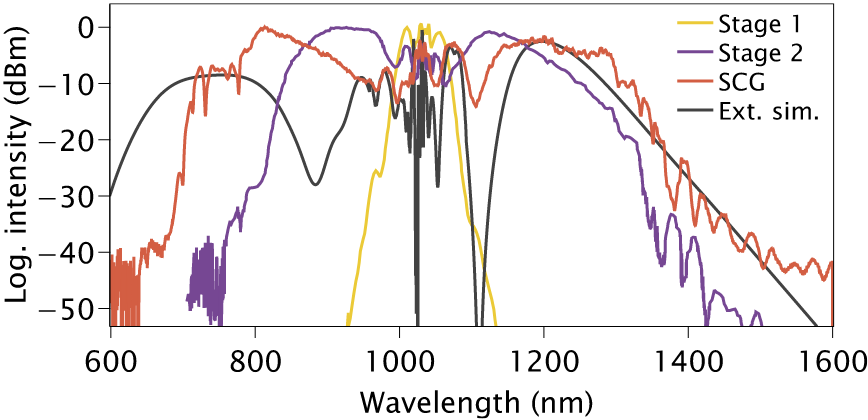
\includegraphics[width=0.5\textwidth]{p6.png}
    \caption{总结工作中的输出光谱: 黄色和紫色分别对应第 1 级和第 2 级输出光谱。橙色对应第2级反常色散下产生超连续谱 (SCG)。灰色是模拟的 SCG，假设腔镜的光谱扩展特性。}\label{p3.3.1}
\end{figure}

%--------------------  附录  --------------------%



\newpage

\appendix
\appendixpage
\addappheadtotoc
\renewcommand{\appendixname}{Appendix\Alph{section}}

\numberwithin{equation}{section}             %%%%%% 公式编号
\numberwithin{figure}{section}            %%%%%% 图片编号

\section{光谱空间均匀性表征} \label{secA}

通过测量压缩光束横向轮廓上的光谱来表征光谱展宽的均匀性，光束准直直径 $2\omega_x\times 2\omega_y$. 

用带有 FC/PC 尖端的多模光纤（400 μm 纤芯直径）沿两个横轴以 0.15 mm 的步长扫描整个光束轮廓，并使用光谱分析仪记录光谱。 

每个光谱 $I(\lambda)$ 与光束轴上的光谱 $I_0(\lambda)$ 的重叠计算为:
\begin{equation}
    V=\frac{[\int (I(\lambda)\cdot I_0(\lambda)\mathrm{d}\lambda)]^2}{\int (I(\lambda)\mathrm{d}\lambda\cdot \int I_0(\lambda)\mathrm{d}\lambda)}
    \label{eq:A.1}
\end{equation}

通过用强度对重叠进行加权，可计算出有效重叠。


%--------------------  插入参考文献  --------------------%

\newpage

\clearpage           %%%  “目录”中显示的页码正确, 需要添加 \clearpage
\phantomsection      %%   “目录”中的链接能正确跳转, 需要添加 \phantomsection
\addcontentsline{toc}{section}{参考文献}   %向目录中添加条目, 以章的名义

\bibliography{ref}

\end{document}